\part{Giao diện SPA, Đặc tả API và Triển khai Docker}
\label{part:ch5}

Chương này trình bày tầng giao tiếp người dùng và hạ tầng vận hành của \texttt{bigdata\_inventory}. Mục~\ref{sec:ch5-ui} mô tả thiết kế ứng dụng React 18 SPA và kỹ thuật bọc biểu đồ Chart.js. Mục~\ref{sec:ch5-api} đặc tả đầy đủ $12$ điểm cuối REST API cùng quy tắc kiểm tra hợp lệ đầu vào. Mục~\ref{sec:ch5-docker} trình bày cấu trúc đóng gói đa container bằng Docker Compose và cấu hình ủy quyền ngược Nginx.

\section{Thiết kế giao diện React 18 SPA và Chart.js}
\label{sec:ch5-ui}
Giao diện người dùng được xây dựng bằng React 18, Vite 5 và Tailwind CSS theo phong cách bảng điều khiển phân tích định lượng: bề mặt nền sáng (\texttt{\#F8FAFC}), thanh điều hướng bên trái tông xám đen đậm (\texttt{\#0F172A}, hỗ trợ thu gọn trên \texttt{Sidebar.jsx}), phông chữ giao diện \textit{Inter} kết hợp phông đơn cách \textit{JetBrains Mono} (\texttt{tabular-nums}) cho các trường mã cửa hàng, mốc thời gian và số liệu định lượng. Thanh tiêu đề \texttt{Header.jsx} hiển thị trạng thái kết nối thời gian thực (\texttt{ENGINE READY | 410,506 rows}) đồng bộ mỗi $5$ giây qua \texttt{/api/health}. Hệ thống tổ chức thành ba thẻ tương tác độc lập:
\begin{itemize}[topsep=0pt, itemsep=1pt]
	\item \textbf{EdaTab.jsx (Hình~\ref{fig:ui-tab1-eda}):} Kết hợp bảng luồng giao dịch trực tiếp (\texttt{SalesStreamTable}, có nút \textit{Tạm dừng/Tiếp tục} và \textit{Xóa bộ đệm}) cùng lưới $2 \times 2$ cho $4$ biểu đồ Chart.js: \texttt{LineChart} (doanh thu theo tháng), \texttt{BarChart} ngang (top $10$ danh mục), \texttt{DoughnutChart} (cơ cấu kênh) và \texttt{BarChart} dọc (tỷ lệ hoàn trả).
	\item \textbf{ForecastTab.jsx (Hình~\ref{fig:ui-tab2-forecast}):} Thanh cấu hình gồm $2$ danh sách chọn (\textit{Product Category}, \textit{Store ID}) nạp từ API, ô nhập số kỳ ($4$--$24$), biểu đồ đường kép so sánh Normal xanh dương (\texttt{\#1D4ED8}) vs. Super cam (\texttt{\#D97706}) và bảng đối soát \texttt{ForecastDiffTable}.
	\item \textbf{InventoryTab.jsx (Hình~\ref{fig:ui-tab3-inventory}):} Biểu đồ \texttt{DoughnutChart} tích lũy ($68\%$ cutout, có nút \textit{Đặt lại}), $3$ thẻ KPI nền trắng viền trái phân biệt trạng thái (\textit{Healthy} xanh lá, \textit{Low Stock} cam, \textit{Overstock} đỏ) kèm thanh tiến trình tỷ trọng, thanh tổng số bản ghi đã xử lý và bảng \texttt{InventoryAlertsTable}.
\end{itemize}

Các thành phần biểu đồ (\texttt{LineChart.jsx}, \texttt{BarChart.jsx}, \texttt{DoughnutChart.jsx}) quản lý vòng đời canvas thông qua \texttt{useRef} và \texttt{useEffect}: trước khi khởi tạo biểu đồ mới hoặc khi component bị gỡ bỏ, hàm dọn dẹp chủ động gọi \texttt{chartInstanceRef.current.destroy()} (hoặc cập nhật tại chỗ \texttt{update('none')} cho biểu đồ tròn tích lũy) để tránh lỗi rò rỉ bộ nhớ và nhấp nháy khung hình.

\begin{figure}[H]
	\centering
	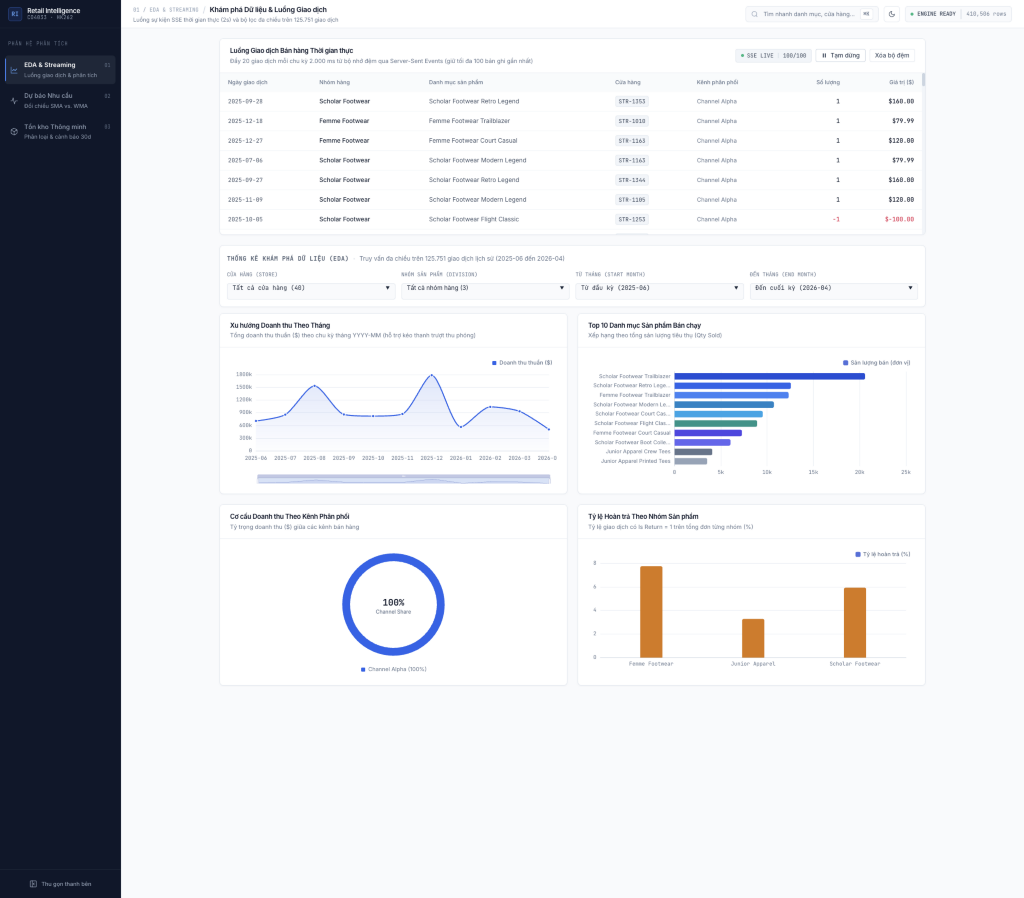
\includegraphics[width=0.95\linewidth]{images/tab1_eda.png}
	\caption{Giao diện Thẻ 1 (\textbf{EDA \& Streaming}): luồng giao dịch trực tiếp và $4$ biểu đồ khám phá dữ liệu}
	\label{fig:ui-tab1-eda}
\end{figure}

\begin{figure}[H]
	\centering
	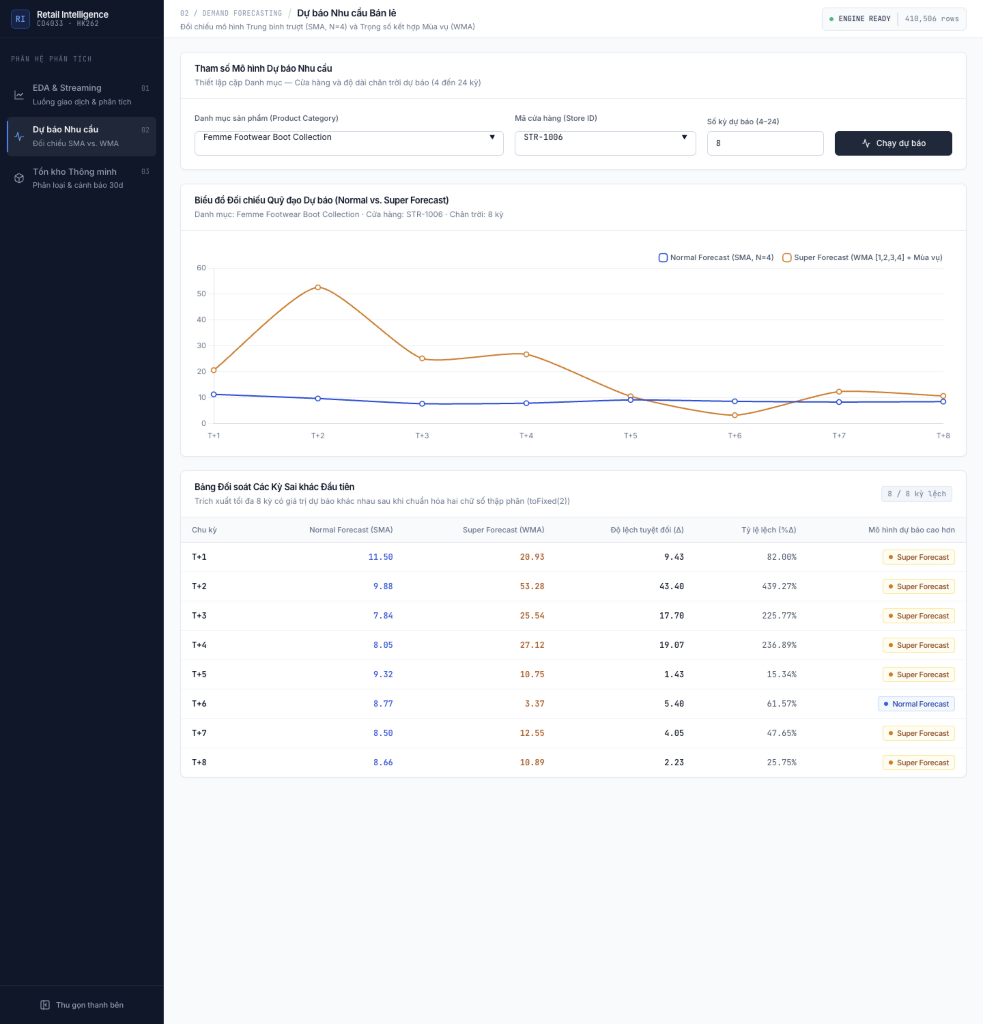
\includegraphics[width=0.95\linewidth]{images/tab2_forecast.png}
	\caption{Giao diện Thẻ 2 (\textbf{Dự báo Nhu cầu}): biểu đồ đối chiếu SMA vs. WMA + Mùa vụ và bảng $8$ kỳ sai khác}
	\label{fig:ui-tab2-forecast}
\end{figure}

\begin{figure}[H]
	\centering
	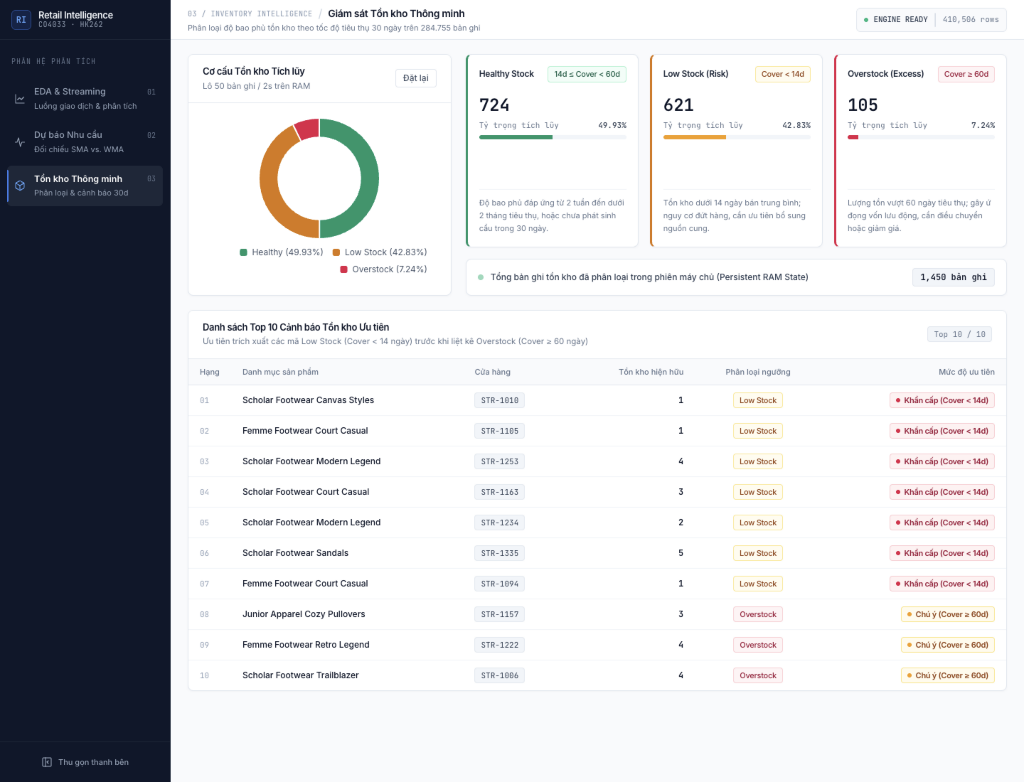
\includegraphics[width=0.95\linewidth]{images/tab3_inventory.png}
	\caption{Giao diện Thẻ 3 (\textbf{Tồn kho Thông minh}): biểu đồ tròn tích lũy, $3$ thẻ KPI và Top $10$ cảnh báo ưu tiên}
	\label{fig:ui-tab3-inventory}
\end{figure}

\section{Đặc tả đầy đủ REST API và Xử lý lỗi tập trung}
\label{sec:ch5-api}
Tầng giao tiếp backend tuân thủ kiến trúc REST~\cite{fielding2000rest}, toàn bộ $12$ điểm cuối được gắn dưới tiền tố \texttt{/api} trong \texttt{backend/routes/index.js} (Bảng~\ref{tab:api-spec}).

\begin{table}[H]
	\centering
	\footnotesize
	\setlength{\tabcolsep}{4pt}
	\begin{tabular}{c l l p{6cm}}
		\toprule
		\textbf{Method} & \textbf{Endpoint}                 & \textbf{Controller}          & \textbf{Chức năng và dữ liệu trả về}                                                        \\
		\midrule
		\texttt{GET}    & \texttt{/api/health}              & \texttt{healthController}    & Trạng thái \texttt{ready}/\texttt{loading}, tổng dòng sales/inventory, \texttt{cumulative}. \\
		\texttt{GET}    & \texttt{/api/stream/sales}        & \texttt{streamController}    & Mảng $20$ giao dịch ngẫu nhiên chưa trùng lặp trong lô.                                     \\
		\texttt{GET}    & \texttt{/api/eda/revenue-trend}   & \texttt{edaController}       & Chuỗi doanh thu theo tháng \texttt{YYYY-MM} đã sắp xếp.                                     \\
		\texttt{GET}    & \texttt{/api/eda/top-categories}  & \texttt{edaController}       & Top $10$ danh mục có \texttt{Qty Sold} cao nhất.                                            \\
		\texttt{GET}    & \texttt{/api/eda/channel-split}   & \texttt{edaController}       & Doanh thu và phần trăm theo \texttt{Sales Channel}.                                         \\
		\texttt{GET}    & \texttt{/api/eda/return-rate}     & \texttt{edaController}       & Số đơn hoàn trả, tổng đơn và tỷ lệ (\%) theo \texttt{Product Division}.                     \\
		\texttt{GET}    & \texttt{/api/forecast/categories} & \texttt{forecastController}  & Danh sách $27$ danh mục duy nhất (có alias \texttt{/api/categories}).                       \\
		\texttt{GET}    & \texttt{/api/forecast/stores}     & \texttt{forecastController}  & Danh sách $40$ mã cửa hàng duy nhất (có alias \texttt{/api/stores}).                        \\
		\texttt{POST}   & \texttt{/api/forecast}            & \texttt{forecastController}  & Nhận \texttt{\{category, store, periods\}} ($4$--$24$), trả 2 chuỗi và tối đa $8$ sai khác. \\
		\texttt{GET}    & \texttt{/api/inventory/stream}    & \texttt{inventoryController} & Cộng dồn lô $50$ bản ghi vào \texttt{\_cumulativeState} và trả tổng tích lũy.               \\
		\texttt{GET}    & \texttt{/api/inventory/alerts}    & \texttt{inventoryController} & Trả danh sách Top $10$ cảnh báo tồn kho ưu tiên \textit{Low Stock}.                         \\
		\texttt{POST}   & \texttt{/api/inventory/reset}     & \texttt{inventoryController} & Đặt lại bộ đếm \texttt{\_cumulativeState} về $\{0, 0, 0, 0\}$.                              \\
		\bottomrule
	\end{tabular}
	\caption{Đặc tả các điểm cuối REST API của hệ thống}
	\label{tab:api-spec}

\end{table}

Trong \texttt{forecastController.js}, yêu cầu \texttt{POST /api/forecast} kiểm tra nghiêm ngặt thân yêu cầu: từ chối với mã \texttt{HTTP 400} nếu không phải đối tượng JSON thuần (\texttt{[object Object]}), \texttt{category} hoặc \texttt{store} rỗng hay vượt quá $200$ ký tự, hoặc \texttt{periods} không phải số nguyên trong đoạn $[4, 24]$. Thân yêu cầu vượt giới hạn $100\text{ KB}$ của \texttt{express.json} nhận mã \texttt{413 PAYLOAD\_TOO\_LARGE}, các tuyến không tồn tại dưới \texttt{/api/*} đi qua bộ bắt \texttt{404 NOT\_FOUND}, và mọi ngoại lệ được \texttt{errorHandler.js} chuẩn hóa theo cấu trúc \texttt{\{success: false, error: \{code, message\}\}} (chỉ kèm \texttt{stack} ở môi trường phát triển khi mã lỗi $\ge 500$).

\section{Đóng gói đa container với Docker Compose và Nginx}
\label{sec:ch5-docker}
Hệ thống triển khai hoàn chỉnh bằng một lệnh \texttt{docker compose up --build -d} với hai dịch vụ kết nối trên mạng cầu nối nội bộ \texttt{inventory-net} (Hình~\ref{fig:docker_topology}):
\begin{itemize}[topsep=0pt, itemsep=1pt]
	\item \textbf{Container backend (\texttt{bigdata\_inventory\_backend}, \texttt{Dockerfile.backend}):} Dựng từ \texttt{node:18-alpine}, chỉ cài phụ thuộc sản xuất (\texttt{npm install --production}), sao chép \texttt{backend/}, \texttt{algorithms/}, \texttt{data/} và \texttt{test\_endpoints.js}. Lệnh \texttt{HEALTHCHECK} mỗi $5$ giây truy vấn địa chỉ IPv4 \texttt{127.0.0.1:3000} tại \texttt{/api/health} thay vì \texttt{localhost} nhằm tránh lỗi \texttt{ECONNREFUSED ::1} trên IPv6 của Alpine Linux.
	\item \textbf{Container frontend (\texttt{bigdata\_inventory\_frontend}, \texttt{Dockerfile} hai giai đoạn):} Giai đoạn $1$ dùng \texttt{node:18-alpine} chạy \texttt{npm run build} để đóng gói Vite; giai đoạn $2$ dọn thư mục Nginx nhưng giữ lại trang lỗi \texttt{50x.html}, sao chép \texttt{dist/} sang \texttt{nginx:alpine} và chỉ khởi chạy khi container backend đạt trạng thái \texttt{service\_healthy}.
\end{itemize}

\begin{figure}[H]
	\centering
	\mermaidfile[width=0.95\linewidth, keepaspectratio]{diagrams/docker_topology.mmd}
	\caption{Kiến trúc triển khai đa container Docker Compose và mạng \texttt{inventory-net}}
	\label{fig:docker_topology}
\end{figure}

Tệp cấu hình \texttt{nginx.conf} (Mã nguồn~\ref{lst:nginx-proxy}) bật nén \texttt{gzip} cho tài nguyên tĩnh và JSON, cấu hình định tuyến SPA (\texttt{try\_files \$uri \$uri/ /index.html}), đồng thời thiết lập thời gian chờ $90\text{ s}$ và bộ đệm $256\text{ k}$ cho tuyến ủy quyền ngược \texttt{/api/} sang \texttt{http://backend:3000/api/}.

\begin{listing}[H]
	\begin{minted}[fontsize=\footnotesize, linenos, breaklines]{nginx}
location / {
    try_files $uri $uri/ /index.html;
}

location /api/ {
    proxy_pass http://backend:3000/api/;
    proxy_http_version 1.1;
    proxy_set_header Host $host;
    proxy_set_header X-Real-IP $remote_addr;
    proxy_connect_timeout 90s;
    proxy_send_timeout 90s;
    proxy_read_timeout 90s;
    proxy_buffer_size 128k;
    proxy_buffers 4 256k;
}
\end{minted}
	\caption{Cấu hình định tuyến SPA và Reverse Proxy trong \texttt{nginx.conf}}
	\label{lst:nginx-proxy}
\end{listing}
